\documentclass[tikz,border=5pt]{standalone}
\usepackage{verbatim}
\usetikzlibrary{shadings,intersections}

\begin{document}
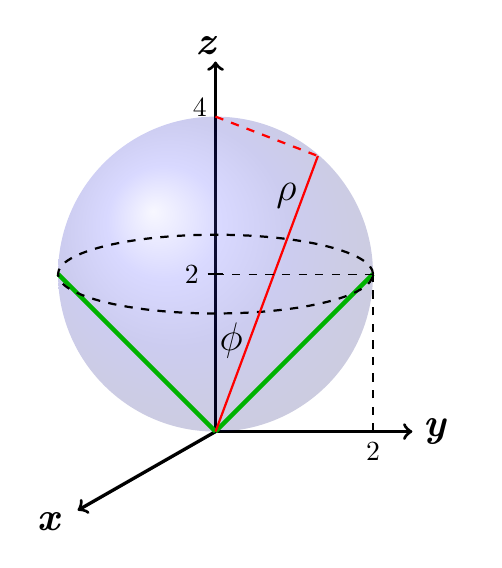
\begin{tikzpicture}

% \coordinate (O) at (0,0);
  \draw [very thick, ->] (0, 0) -- (2.5, 0);
  \draw [very thick, ->] (0, 0) -- (-1.75, -1);
  \draw [very thick, ->] (0, 0) -- (0, 4.7);

  \shade[ball color = blue, opacity = 0.2] (0,2) circle (2);
  \draw [ultra thick, black!30!green] (0, 0) -- (2, 2) ;
  \draw [ultra thick, black!30!green] (0, 0) -- (-2, 2) ;
 \draw [ thick, dashed] (0, 2) ellipse (2 and .5);

 \draw [thick, red] (0, 0) -- (1.3, 3.5);
 \draw [thick, red, dashed] (0, 4) -- (1.3, 3.5);

  \draw [ thick] (-.1, 2) -- (.1, 2) ;
  \draw (-.3, 2) node {2};
  \draw (.9, 3) node { \Large $\rho$ } ;
  \draw [thick, dashed] (2, 0) -- (2, 2) ;
  \draw (2, -.25) node {2};
  \draw (-.2, 4.12) node {4} ;
  \draw [dashed] (0, 2) -- (2, 2) ;

  \draw (.2, 1.15) node { \Large $\phi$ } ;

  \draw (-2, -1.15) node { \Large \textbf  {\textit x } } ;	
  \draw (2.9, 0) node { \Large \textbf  {\textit y } } ;	
  \draw (0, 4.9) node { \Large \textbf  {\textit z } } ;	

\end{tikzpicture}
\end{document}
